\documentclass[12pt]{article}

\usepackage[provide=*,spanish]{babel}
\usepackage[utf8]{inputenc}
\usepackage[T1]{fontenc}
\usepackage{graphicx}
\usepackage{xcolor}
\usepackage{amsmath}
\usepackage{tikz}
\usetikzlibrary{arrows.meta,positioning,shapes.geometric,calc}
\usepackage{float}
\usepackage{enumitem}
\usepackage{array}
\usepackage{booktabs}
\usepackage{subcaption}
\usepackage{fancyhdr}
\usepackage[a4paper,margin=2.5cm]{geometry}
\usepackage[hidelinks]{hyperref}

\renewcommand{\arraystretch}{1.3}

% -------- ENCABEZADO --------
\setlength{\headheight}{15pt}
\pagestyle{fancy}
\fancyhf{}
\lhead{\small Laboratorio de Sistemas de Comunicaciones}
\rhead{\small Práctica No.\ 7}
\cfoot{\thepage}

\begin{document}

% ========================
%        PORTADA
% ========================
\begin{titlepage}
\centering

% -------- LOGOS Y ENCABEZADO --------
\begin{minipage}[c]{0.18\textwidth}
\centering

\includegraphics[width=\textwidth]{imagenes/unam.png}
\end{minipage}
\begin{minipage}[c]{0.60\textwidth}
\centering
{\Large \textbf{UNIVERSIDAD NACIONAL AUTÓNOMA DE MÉXICO}\par}
\vspace{0.4cm}
{\Large \textbf{FACULTAD DE INGENIERÍA}\par}
\end{minipage}
\begin{minipage}[c]{0.18\textwidth}
\centering

\includegraphics[width=\textwidth]{imagenes/fi.png}
\end{minipage}

\vspace{1.8cm}

% -------- ASIGNATURA --------
Asignatura:\\[0.2cm]
{\Large \textit{\textbf{Laboratorio de Sistemas de Comunicaciones}}\par}

\vspace{1.2cm}

% -------- REPORTE Y PRACTICA --------
\textbf{Reporte de la Práctica} No.\ 7\\[0.2cm]
Distorsión Alineal

\vspace{1.2cm}

% -------- INTEGRANTES --------
Integrantes:\\[0.2cm]
Díaz Antúnez David\\
Escribano Tepox Jennifer del Rocío\\
Parra Bello Carlos Enrique

\vspace{1.2cm}

% -------- PROFESORES --------
Profesor de laboratorio\\
Ing.\ José Alberto López Cervantes\\
Grupo: 16

\vspace{1.2cm}

% -------- FECHA Y SEMESTRE --------
Fecha de entrega:\\
02/11/2026

\vspace{0.6cm}

Semestre 2027-1

\vfill

\hfill \textit{Calificación}: \rule{3.5cm}{0.4pt} \hspace{0.3cm}

\end{titlepage}

\tableofcontents
\newpage

% ========================
%        OBJETIVOS
% ========================
\section{Objetivos}

El alumno:

\begin{enumerate}[label=\arabic*.]
    \item Analizará la influencia de los elementos eléctricos y electrónicos no lineales en la transmisión de señales de comunicaciones, evaluando sus efectos en la calidad de la señal.
    \item Identificará los diferentes tipos de distorsión no lineal.
    \item Observará la respuesta de dispositivos no lineales ante señales de diferente nivel de amplitud.
    \item Cuantificará la distorsión alineal por armónicos.
    \item Observará la generación de productos de intermodulación.
    \item Observará la respuesta de dispositivos no lineales ante señales de diferente amplitud.
    \item Conocerá que los dispositivos alineales pueden tener aplicaciones de gran utilidad.
\end{enumerate}

% ========================
%      EXPERIMENTOS
% ========================
\section{Lista de experimentos}

\begin{enumerate}[label=\arabic*.]
    \item Verificación de la alinealidad del circuito utilizado.
    \item Obtención y medición de la distorsión armónica.
    \item Observación de la distorsión por intermodulación.
\end{enumerate}

% ========================
%      LISTA DE EQUIPO
% ========================
\section{Lista de equipo}

\begin{itemize}[label=--]
    \item Multímetro
    \item Osciloscopio
    \item Analizador de espectros
    \item 2 Generadores de funciones
    \item Amplificador de señal pequeña
    \item Fuente de alimentación de DC
\end{itemize}

% ========================
%   INTRODUCCIÓN TEÓRICA
% ========================
\section{Introducción teórica}

\subsection*{Sistemas lineales y no lineales}

Un sistema es lineal cuando cumple el principio de superposición: si a las entradas $x_1(t)$ y $x_2(t)$ les corresponden las salidas $y_1(t)$ y $y_2(t)$, entonces a la entrada $\alpha x_1(t) + \beta x_2(t)$ le corresponde la salida $\alpha y_1(t) + \beta y_2(t)$. Una consecuencia directa es que un sistema lineal e invariante en el tiempo \emph{no crea frecuencias nuevas}: sólo puede modificar la amplitud y la fase de las componentes ya presentes en la entrada.

En la práctica, ningún dispositivo electrónico es perfectamente lineal. Diodos, transistores y amplificadores operacionales presentan una característica de transferencia $y = f(x)$ que sólo es aproximadamente recta en un intervalo limitado de amplitudes; fuera de él aparecen fenómenos como la saturación, el corte o la zona muerta (Figura~\ref{fig:transferencia}). Cuando la señal excursiona por estas regiones, la salida deja de ser una réplica escalada de la entrada y se dice que el sistema introduce \textbf{distorsión no lineal} o \textbf{alineal}.

\begin{figure}[H]
\centering
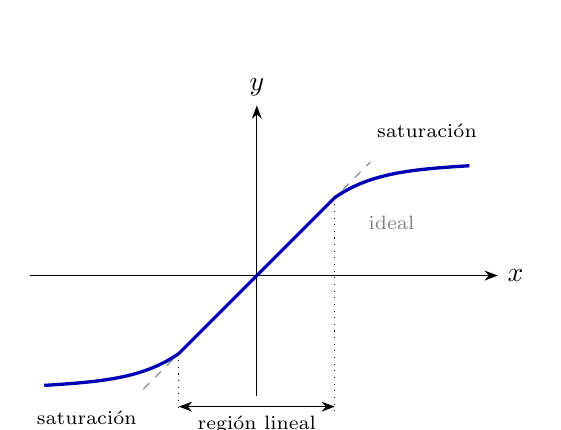
\begin{tikzpicture}[>=Stealth, scale=0.9]
    \draw[->] (-3.2,0) -- (3.4,0) node[right] {$x$};
    \draw[->] (0,-1.7) -- (0,2.4) node[above] {$y$};
    \draw[dashed, gray] (-1.6,-1.6) -- (1.6,1.6);
    \draw[very thick, blue!70!black]
        (-3,-1.55) .. controls (-2.2,-1.5) and (-1.6,-1.45) .. (-1.1,-1.1)
        -- (1.1,1.1) .. controls (1.6,1.45) and (2.2,1.5) .. (3,1.55);
    \draw[dotted] (-1.1,-1.1) -- (-1.1,-1.9) (1.1,1.1) -- (1.1,-1.9);
    \draw[<->] (-1.1,-1.85) -- (1.1,-1.85) node[midway, below, font=\scriptsize] {región lineal};
    \node[font=\scriptsize, align=center] at (2.4,2.05) {saturación};
    \node[font=\scriptsize, align=center] at (-2.4,-2.0) {saturación};
    \node[font=\scriptsize, gray] at (1.9,0.75) {ideal};
\end{tikzpicture}
\caption{Característica de transferencia de un amplificador con saturación.}
\label{fig:transferencia}
\end{figure}

\subsection*{Modelo por serie de potencias}

Un dispositivo no lineal sin memoria puede modelarse alrededor de su punto de operación mediante una serie de potencias:
\[
y(t) = a_1 x(t) + a_2 x^2(t) + a_3 x^3(t) + \cdots
\]
donde $a_1$ es la ganancia lineal y los coeficientes $a_2, a_3, \ldots$ cuantifican la alinealidad. Si la entrada es un tono $x(t) = A\cos(\omega_1 t)$, al usar las identidades $\cos^2\theta = \tfrac{1}{2}(1+\cos 2\theta)$ y $\cos^3\theta = \tfrac{1}{4}(3\cos\theta + \cos 3\theta)$ se obtiene:
\[
y(t) = \frac{a_2A^2}{2} + \left(a_1A + \frac{3a_3A^3}{4}\right)\cos\omega_1 t + \frac{a_2A^2}{2}\cos 2\omega_1 t + \frac{a_3A^3}{4}\cos 3\omega_1 t + \cdots
\]
Es decir, aparecen una componente de directa y \textbf{armónicos} en múltiplos enteros de la frecuencia de entrada. Los términos de orden par ($a_2, a_4, \ldots$) generan armónicos pares y están asociados a características de transferencia asimétricas; los de orden impar ($a_3, a_5, \ldots$) generan armónicos impares, propios de recortes simétricos. Además, la amplitud de cada armónico crece más rápido que la de la fundamental ($A^2$, $A^3$, \ldots), por lo que la distorsión aumenta con el nivel de la señal de entrada.

\subsection*{Clasificación de la distorsión alineal}

\begin{itemize}[label=--]
    \item \textbf{Distorsión armónica:} generación de componentes en $n f_1$ ($n = 2, 3, \ldots$) cuando la entrada es un solo tono de frecuencia $f_1$.
    \item \textbf{Distorsión por intermodulación:} cuando la entrada contiene dos o más tonos, $f_1$ y $f_2$, la alinealidad genera además componentes en las frecuencias suma y diferencia
    \[
    f_{IM} = |m f_1 \pm n f_2|, \qquad m, n = 0, 1, 2, \ldots
    \]
    cuyo orden es $m + n$. Por ejemplo, el término $a_2x^2$ produce $f_2 \pm f_1$ y el término $a_3x^3$ produce $2f_1 \pm f_2$ y $2f_2 \pm f_1$. Los productos de tercer orden son los más perjudiciales en comunicaciones porque pueden caer dentro de la banda de la señal útil.
    \item \textbf{Compresión de ganancia:} cerca de la saturación la ganancia efectiva para la fundamental disminuye y la salida deja de crecer proporcionalmente con la entrada.
    \item \textbf{Distorsión por recorte y por cruce:} el recorte ocurre cuando la señal alcanza los límites de alimentación del amplificador; la distorsión por cruce aparece en etapas de salida clase B alrededor del paso por cero.
\end{itemize}

\subsection*{Cuantificación de la distorsión armónica}

La distorsión armónica total (THD, \emph{Total Harmonic Distortion}) compara el valor eficaz del contenido armónico con el de la fundamental:
\[
\%D = \frac{\sqrt{V_2^2 + V_3^2 + V_4^2 + \cdots}}{V_1}\times 100\,\%
\]
Como, por el teorema de Parseval, el cuadrado del valor eficaz total de una señal periódica es la suma de los cuadrados de los valores eficaces de sus componentes, $V_T^2 = V_1^2 + V_2^2 + V_3^2 + \cdots$, la expresión anterior puede evaluarse midiendo sólo $V_T$ con un multímetro de verdadero valor eficaz y $V_1$ con el analizador de espectros:
\[
\%D = \frac{\sqrt{V_T^2 - V_1^2}}{V_1}\times 100\,\%
\]

\subsection*{Efecto de los filtros sobre una señal distorsionada}

Un filtro RC es un sistema lineal, por lo que no genera frecuencias nuevas, pero sí modifica la proporción entre la fundamental y los armónicos. Un filtro pasa-bajas atenúa más los armónicos que la fundamental y \emph{reduce} el porcentaje de distorsión; un filtro pasa-altas atenúa más la fundamental y lo \emph{incrementa}. Para una red RC pasa-altas de primer orden:
\[
|H(f)| = \frac{f/f_c}{\sqrt{1 + (f/f_c)^2}}, \qquad f_c = \frac{1}{2\pi RC}.
\]

\subsection*{Aplicaciones de la alinealidad}

Aunque en un canal de transmisión la alinealidad es indeseable, también es la base de procesos fundamentales en comunicaciones: los mezcladores y moduladores aprovechan el término cuadrático para generar las frecuencias suma y diferencia (conversión de frecuencia, modulación AM), los detectores de envolvente usan la característica del diodo para demodular y los multiplicadores de frecuencia seleccionan un armónico específico mediante un filtro.

% ========================
%   DESARROLLO DE LA PRÁCTICA
% ========================
\section{Desarrollo de la práctica}

\textit{Diagrama de conexiones en bloques. Con ayuda de su profesor, implemente el circuito de la Figura 7.1.}

\begin{figure}[H]
\centering
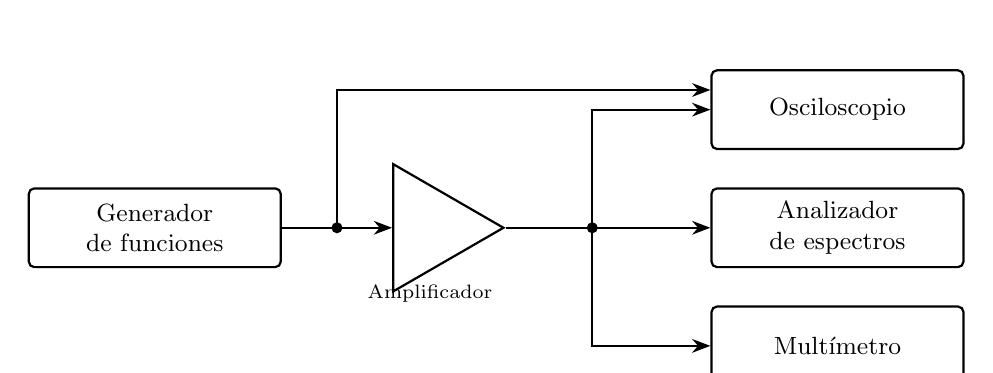
\begin{tikzpicture}[
    blk/.style={draw, thick, rounded corners=2pt, minimum width=3.2cm, minimum height=1cm, align=center, font=\small},
    amp/.style={draw, thick, isosceles triangle, isosceles triangle apex angle=60, minimum height=1.4cm, inner sep=0pt},
    >=Stealth]
    \node[blk] (gen) {Generador\\de funciones};
    \node[amp, right=1.4cm of gen] (amp) {};
    \node[font=\scriptsize, below=0.05cm of amp] {Amplificador};
    \node[blk, right=2.6cm of amp, yshift=1.5cm] (osc) {Osciloscopio};
    \node[blk, right=2.6cm of amp] (esp) {Analizador\\de espectros};
    \node[blk, right=2.6cm of amp, yshift=-1.5cm] (mul) {Multímetro};
    \draw[thick,->] (gen.east) -- (amp.west);
    \coordinate (n) at ($(amp.east)+(1.1,0)$);
    \draw[thick] (amp.east) -- (n);
    \fill (n) circle (2pt);
    \draw[thick,->] (n) |- (osc.west);
    \draw[thick,->] (n) -- (esp.west);
    \draw[thick,->] (n) |- (mul.west);
    \coordinate (m) at ($(gen.east)!0.5!(amp.west)$);
    \fill (m) circle (2pt);
    \draw[thick,->] (m) |- ($(osc.west)+(0,0.25)$);
\end{tikzpicture}
\caption{Diagrama de conexiones en bloques (Figura 7.1 del manual).}
\end{figure}

Para cuantificar la distorsión armónica se utilizó la relación entre el valor eficaz total de la señal de salida, $V_T$ (medido con el multímetro de verdadero valor eficaz), y el valor eficaz de la componente fundamental, $V_1$ (medido con el analizador de espectros):
\[
\%D = \frac{\sqrt{V_2^2 + V_3^2 + V_4^2 + \cdots}}{V_1}\times 100\%
     = \frac{\sqrt{V_T^2 - V_1^2}}{V_1}\times 100\%
\]
donde $V_n$ es el valor eficaz del $n$-ésimo armónico y $V_T^2 = V_1^2 + V_2^2 + V_3^2 + \cdots$ (teorema de Parseval).

% ---------------- ACTIVIDAD 1 ----------------
\subsection{Actividad 1}

\textit{Genere una señal senoidal a 1\,kHz. Consigne en el reporte el oscilograma y el espectro. Anote sus observaciones.}

% Agregar aquí oscilograma, espectro, escalas y observaciones.
% \begin{figure}[H]
% \centering
% \begin{subfigure}{0.48\textwidth}\centering
% \includegraphics[width=\textwidth]{imagenes/act1_osc.jpg}
% \caption{Oscilograma.}
% \end{subfigure}\hfill
% \begin{subfigure}{0.48\textwidth}\centering
% \includegraphics[width=\textwidth]{imagenes/act1_espectro.jpg}
% \caption{Espectro de magnitud.}
% \end{subfigure}
% \caption{Señal senoidal de 1\,kHz a la salida del amplificador.}
% \end{figure}

% ---------------- ACTIVIDAD 2 ----------------
\subsection{Actividad 2}

\textit{Mida y anote la ganancia del amplificador.}

% G =

% ---------------- ACTIVIDAD 3 ----------------
\subsection{Actividad 3}

\textit{Aumente la amplitud de la señal de entrada. Note la distorsión armónica que se produce en la salida. Anote el espectro y oscilograma. Calcule el porcentaje de distorsión de la señal a la salida.}

\begin{figure}[H]
\centering
\begin{subfigure}{0.48\textwidth}\centering
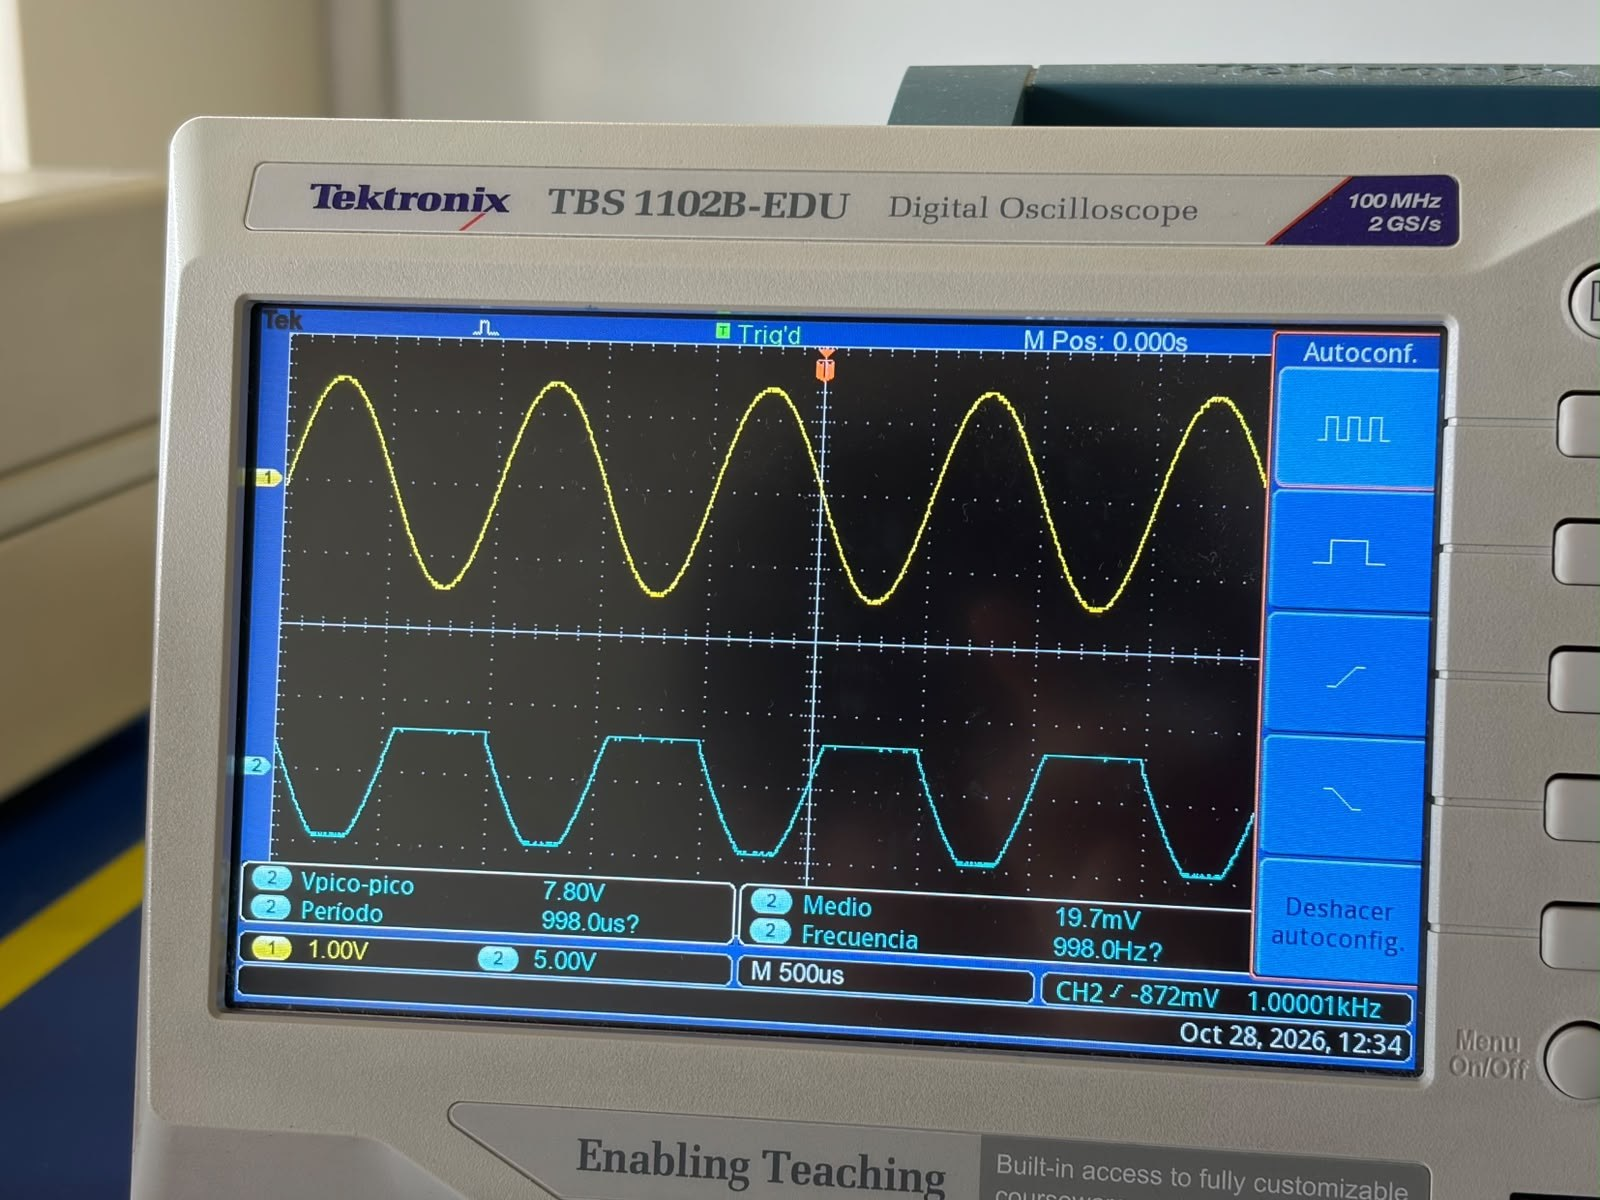
\includegraphics[width=\textwidth]{imagenes/act3_osc.jpg}
\caption{Oscilograma. CH1: entrada; CH2: salida.}
\end{subfigure}\hfill
\begin{subfigure}{0.48\textwidth}\centering
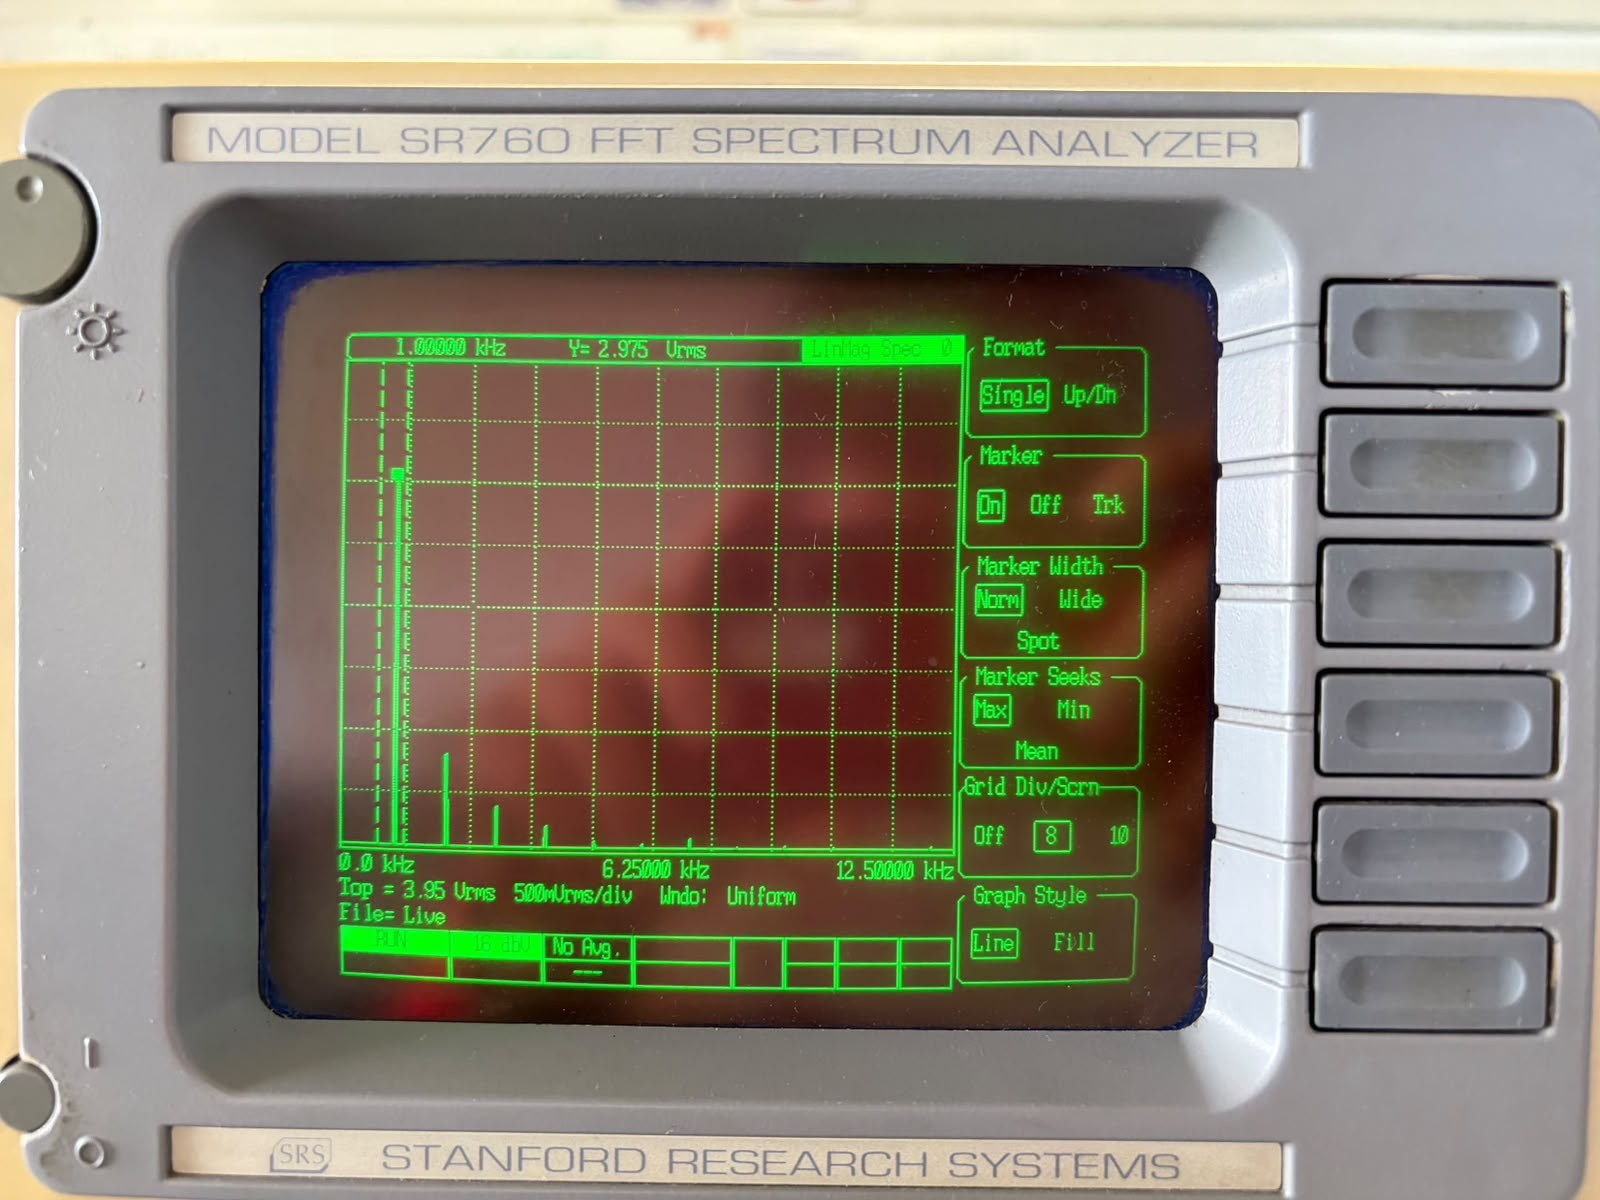
\includegraphics[width=\textwidth]{imagenes/act3_espectro.jpg}
\caption{Espectro de magnitud de la salida.}
\end{subfigure}
\caption{Salida del amplificador con la amplitud de entrada aumentada.}
\end{figure}

\begin{table}[H]
\centering
\begin{tabular}{|l|l|}
\hline
\textbf{Parámetro} & \textbf{Valor} \\ \hline
Escala horizontal & $500\,\mu$s/div \\ \hline
Escala vertical & CH1: $1$ V/div;\; CH2: $5$ V/div \\ \hline
Voltaje pico a pico de salida, $V_{pp}$ & $7.80$ V \\ \hline
Frecuencia de la salida & $1$ kHz \\ \hline
Escala del analizador & $500$ mV$_{RMS}$/div;\; $0$--$12.5$ kHz \\ \hline
Amplitud de la fundamental, $V_1$ & $2.975$ V$_{RMS}$ \\ \hline
Valor eficaz total, $V_T$ & $3.1$ V$_{RMS}$ \\ \hline
\end{tabular}
\caption{Mediciones a la salida del amplificador.}
\end{table}

Cálculo del porcentaje de distorsión:
\[
\begin{aligned}
\%D &= \frac{\sqrt{(3.1)^2 - (2.975)^2}}{2.975}\times 100\%
     = \frac{\sqrt{9.61 - 8.8506}}{2.975}\times 100\%\\
    &= \frac{0.8714}{2.975}\times 100\% = 29.29\%
\end{aligned}
\]

\textbf{Observaciones:} al aumentar la amplitud de la entrada, el amplificador llega a su región de saturación y la salida se recorta: las crestas de la senoide se aplanan y la forma de onda tiende a un trapecio, mientras que la señal de entrada (CH1) permanece senoidal. El recorte no es simétrico (las mesetas positivas son más anchas que las negativas), por lo que en el espectro, además de la fundamental en 1\,kHz, aparecen armónicos pares e impares en 2, 3, 4\,kHz y una componente menor en 7\,kHz, todos múltiplos enteros de la frecuencia de entrada. Ninguna de estas componentes existía en la entrada: son generadas por la característica de transferencia no lineal del amplificador.

% ---------------- ACTIVIDAD 4 ----------------
\subsection{Actividad 4}

\textit{Anote el oscilograma y el espectro de la señal de salida del primer circuito RC. Realice las mediciones necesarias para calcular el porcentaje de distorsión.}

\begin{figure}[H]
\centering
\begin{subfigure}{0.48\textwidth}\centering
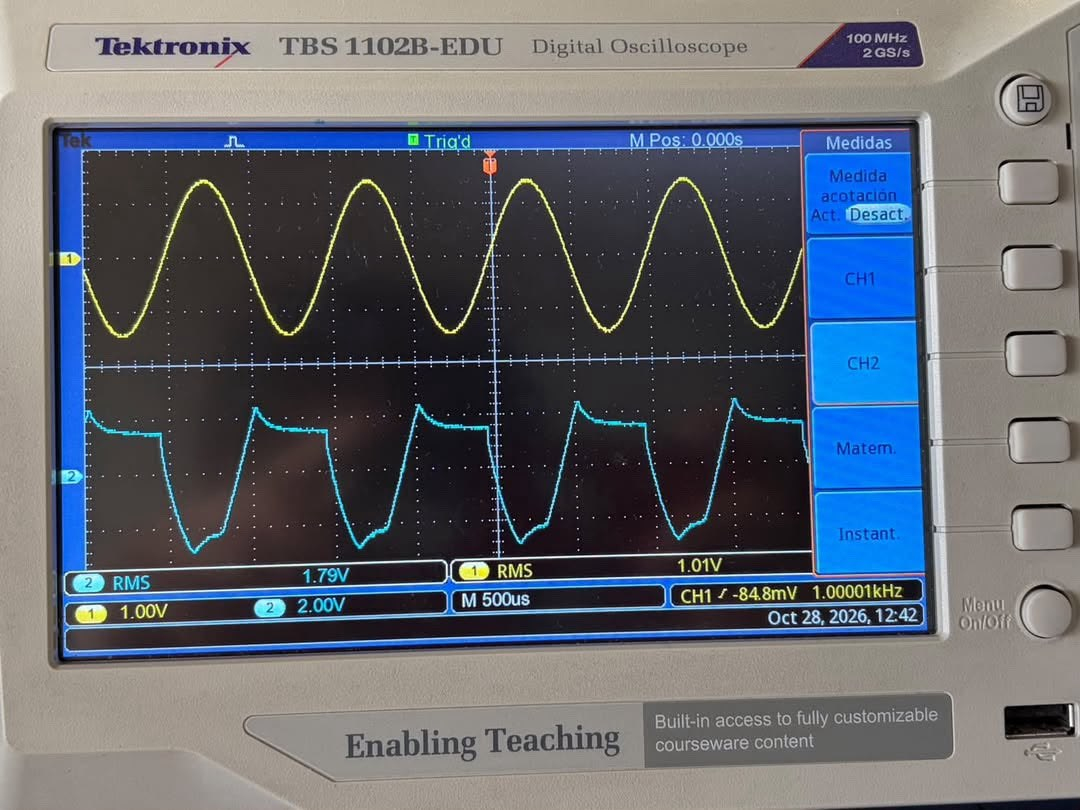
\includegraphics[width=\textwidth]{imagenes/act4_osc.jpg}
\caption{Oscilograma. CH1: entrada; CH2: salida del primer RC.}
\end{subfigure}\hfill
\begin{subfigure}{0.48\textwidth}\centering
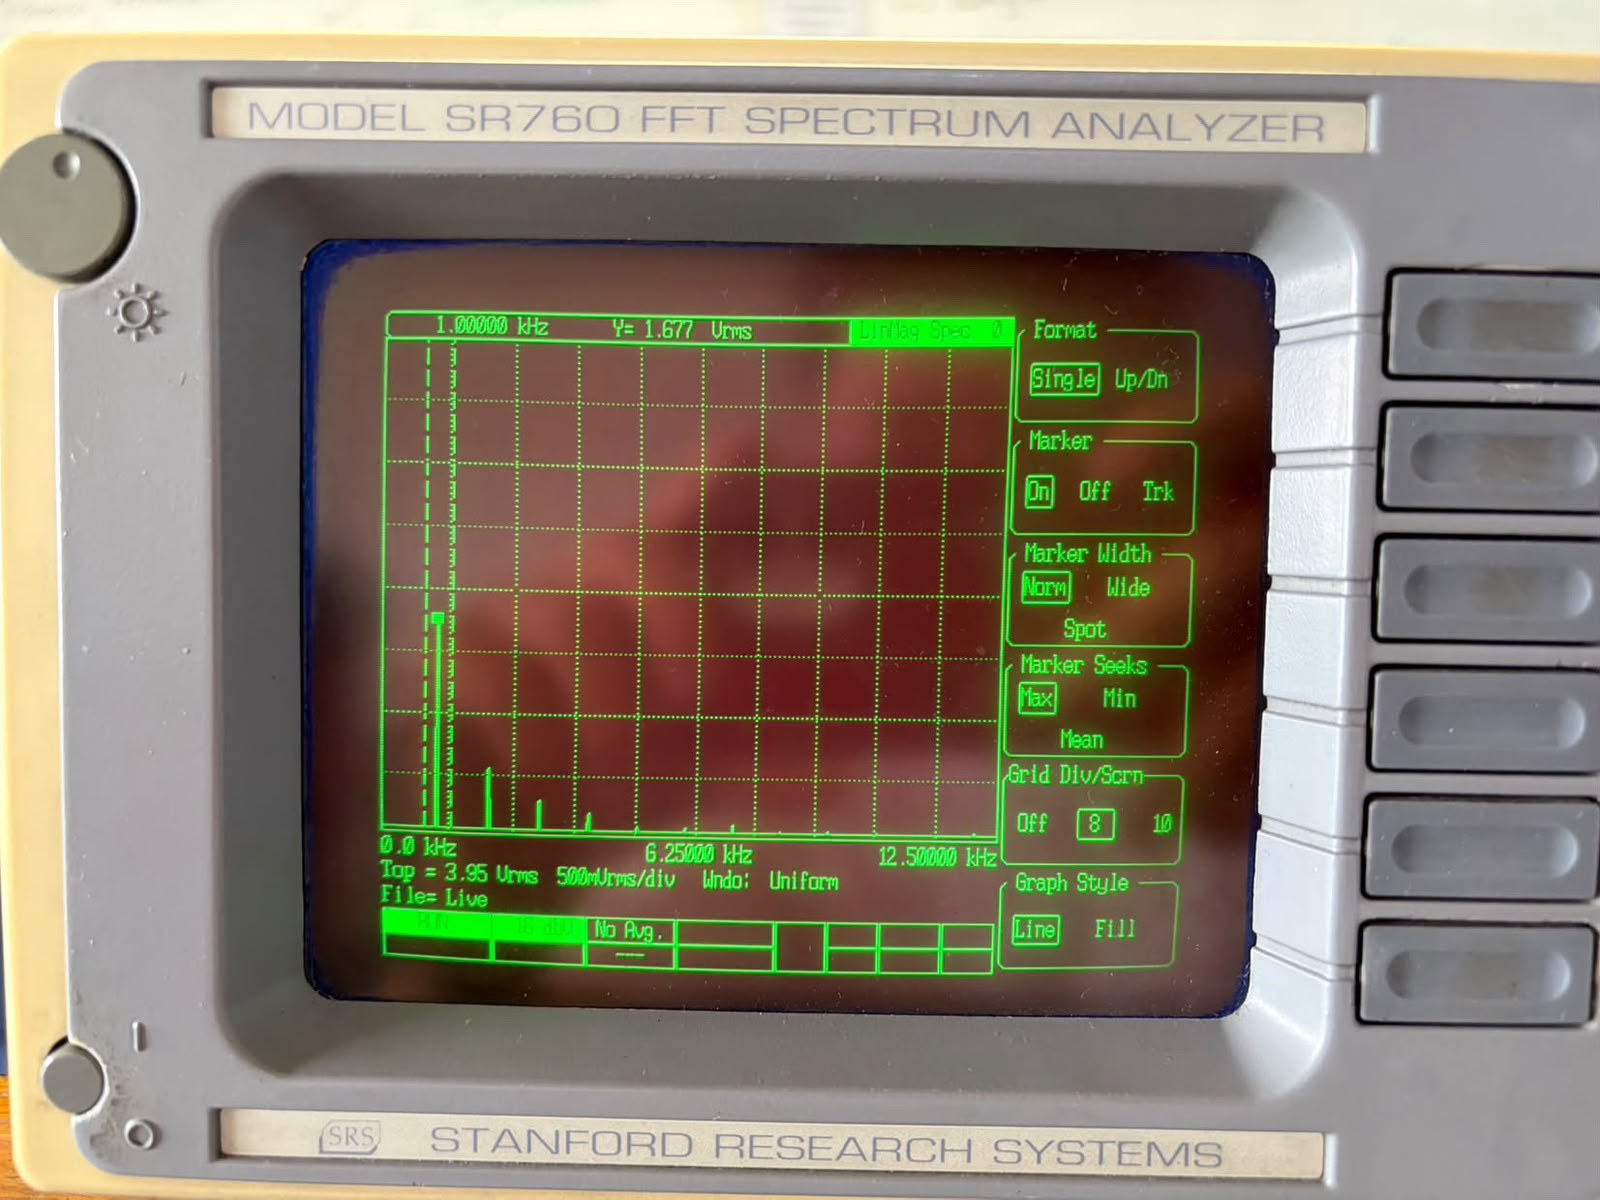
\includegraphics[width=\textwidth]{imagenes/act4_espectro.jpg}
\caption{Espectro de magnitud a la salida del primer RC.}
\end{subfigure}
\caption{Señal a la salida del primer circuito RC.}
\end{figure}

\begin{table}[H]
\centering
\begin{tabular}{|l|l|}
\hline
\textbf{Parámetro} & \textbf{Valor} \\ \hline
Escala horizontal & $500\,\mu$s/div \\ \hline
Escala vertical & CH1: $1$ V/div;\; CH2: $2$ V/div \\ \hline
Valor eficaz de la entrada (CH1) & $1.01$ V$_{RMS}$ \\ \hline
Valor eficaz de la salida (CH2, osciloscopio) & $1.79$ V$_{RMS}$ \\ \hline
Amplitud de la fundamental, $V_1$ & $1.677$ V$_{RMS}$ \\ \hline
Valor eficaz total, $V_T$ (multímetro) & $1.78$ V$_{RMS}$ \\ \hline
\end{tabular}
\caption{Mediciones a la salida del primer circuito RC.}
\end{table}

Cálculo del porcentaje de distorsión:
\[
\begin{aligned}
\%D &= \frac{\sqrt{(1.78)^2 - (1.677)^2}}{1.677}\times 100\%
     = \frac{\sqrt{3.1684 - 2.8123}}{1.677}\times 100\%\\
    &= \frac{0.5967}{1.677}\times 100\% = 35.58\%
\end{aligned}
\]

\textbf{Observaciones:} la forma de onda a la salida del primer RC ya no es un trapecio: después de cada transición aparece un pico seguido de un decaimiento exponencial durante las mesetas, comportamiento característico de una red que responde a la derivada de la señal. La fundamental disminuyó de $2.975$ a $1.677$\,V$_{RMS}$ ($-4.98$\,dB), mientras que los armónicos se atenuaron proporcionalmente menos, de modo que el porcentaje de distorsión aumentó de $29.29\,\%$ a $35.58\,\%$.

% ---------------- ACTIVIDAD 5 ----------------
\subsection{Actividad 5}

\textit{Conecte los instrumentos de medición a la salida del segundo circuito RC, calcule nuevamente el porcentaje de distorsión. Consigne en el reporte las gráficas y los datos numéricos.}

\begin{figure}[H]
\centering
\begin{subfigure}{0.48\textwidth}\centering
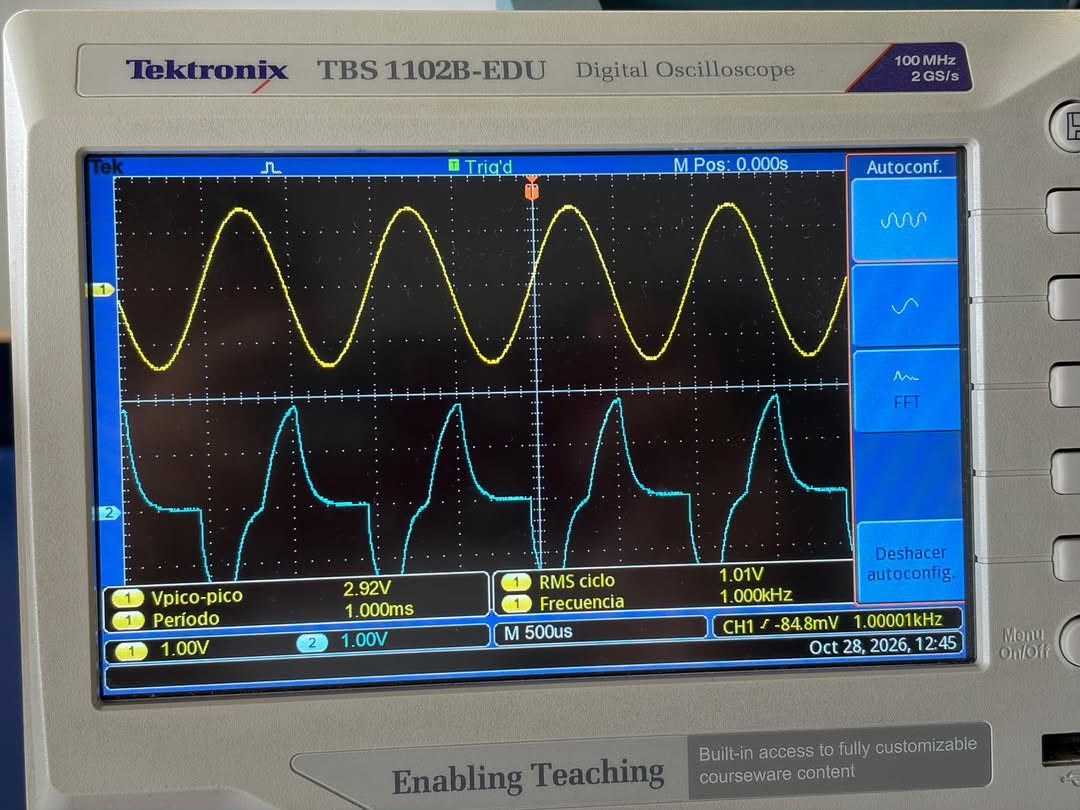
\includegraphics[width=\textwidth]{imagenes/act5_osc.jpg}
\caption{Oscilograma. CH1: entrada; CH2: salida del segundo RC.}
\end{subfigure}\hfill
\begin{subfigure}{0.48\textwidth}\centering
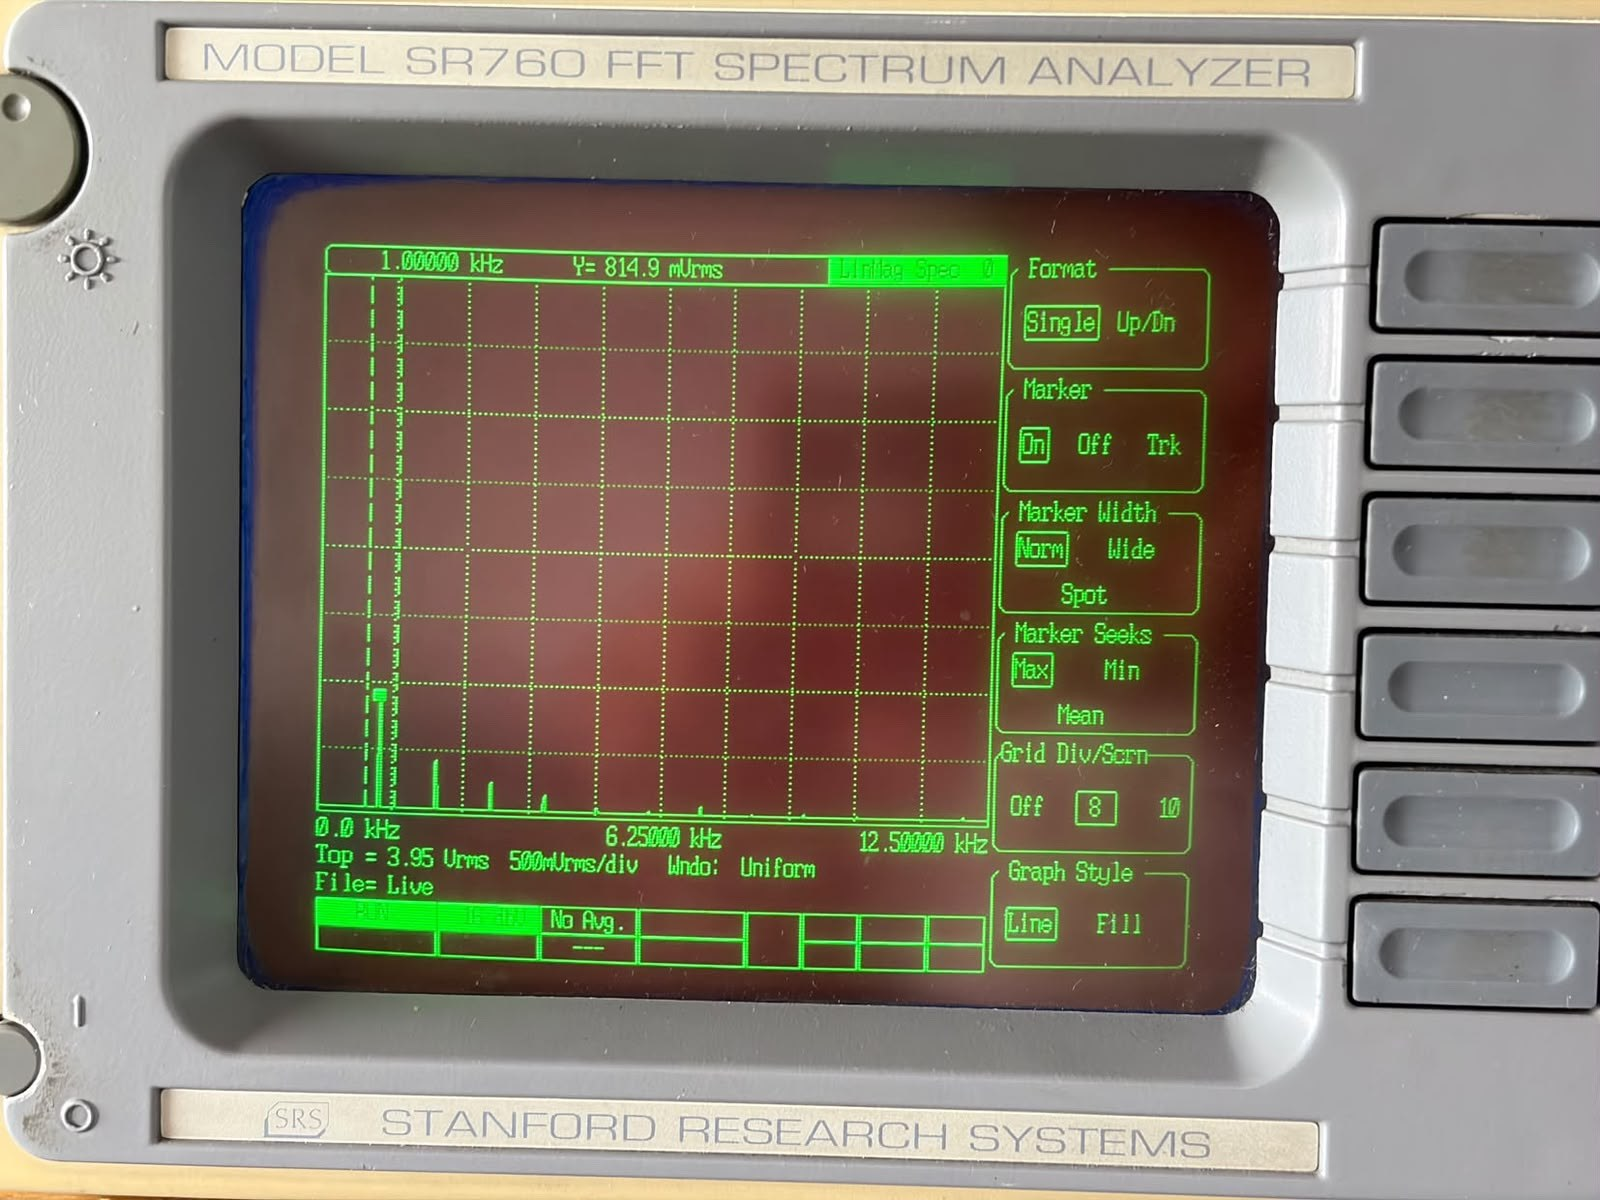
\includegraphics[width=\textwidth]{imagenes/act5_espectro.jpg}
\caption{Espectro de magnitud a la salida del segundo RC.}
\end{subfigure}
\caption{Señal a la salida del segundo circuito RC.}
\end{figure}

\begin{table}[H]
\centering
\begin{tabular}{|l|l|}
\hline
\textbf{Parámetro} & \textbf{Valor} \\ \hline
Escala horizontal & $500\,\mu$s/div \\ \hline
Escala vertical & CH1: $1$ V/div;\; CH2: $1$ V/div \\ \hline
Entrada (CH1) & $2.92$ V$_{pp}$;\; $1.01$ V$_{RMS}$;\; $1$ kHz \\ \hline
Amplitud de la fundamental, $V_1$ & $814.9$ mV$_{RMS}$ \\ \hline
Valor eficaz total, $V_T$ (multímetro) & $935.4$ mV$_{RMS}$ \\ \hline
\end{tabular}
\caption{Mediciones a la salida del segundo circuito RC.}
\end{table}

Cálculo del porcentaje de distorsión:
\[
\begin{aligned}
\%D &= \frac{\sqrt{(0.9354)^2 - (0.8149)^2}}{0.8149}\times 100\%
     = \frac{\sqrt{0.8750 - 0.6641}}{0.8149}\times 100\%\\
    &= \frac{0.4593}{0.8149}\times 100\% = 56.36\%
\end{aligned}
\]

\textbf{Observaciones:} el efecto del primer RC se acentúa: los picos posteriores a cada transición son más pronunciados y la señal se aleja aún más de una senoide. La fundamental cayó de $1.677$ a\ $0.8149$\,V$_{RMS}$ ($-6.27$\,dB) y la distorsión aumentó hasta $56.36\,\%$, casi el doble del valor medido a la salida del amplificador.

% ---------------- ACTIVIDAD 6 ----------------
\subsection{Actividad 6}

\textit{¿Qué función realiza cada circuito RC?}

Cada circuito RC funciona como un \textbf{filtro pasa\nobreakdash-altas de primer orden}, es decir, una red derivadora: el capacitor en serie presenta una reactancia $X_C = 1/(2\pi f C)$ que disminuye al aumentar la frecuencia, por lo que su función de transferencia es
\[
|H(f)| = \frac{f/f_c}{\sqrt{1 + (f/f_c)^2}}, \qquad f_c = \frac{1}{2\pi RC}.
\]
En consecuencia, la fundamental de 1\,kHz se atenúa más que los armónicos de 2, 3 y 4\,kHz; el capacitor en serie además bloquea cualquier componente de directa. Los resultados lo confirman:

\begin{table}[H]
\centering
\begin{tabular}{|l|c|c|c|c|}
\hline
\textbf{Punto de medición} & $V_1$ [V$_{RMS}$] & $V_T$ [V$_{RMS}$] & \textbf{Atenuación de $V_1$} & $\%D$ \\ \hline
Salida del amplificador & $2.975$ & $3.1$ & -- & $29.29\,\%$ \\ \hline
Salida del 1.\textsuperscript{er} RC & $1.677$ & $1.78$ & $-4.98$ dB & $35.58\,\%$ \\ \hline
Salida del 2.\textsuperscript{o} RC & $0.8149$ & $0.9354$ & $-6.27$ dB & $56.36\,\%$ \\ \hline
\end{tabular}
\caption{Evolución de la fundamental y de la distorsión a través de las etapas RC.}
\end{table}

Si los circuitos RC fueran pasa-bajas, atenuarían los armónicos más que la fundamental y la distorsión disminuiría; como ocurrió lo contrario, se concluye que ambas etapas son pasa-altas. Conectadas en cascada forman un filtro pasa-altas de segundo orden ($-40$\,dB/década por debajo de $f_c$), por lo que la segunda etapa incrementa aún más la proporción de armónicos respecto a la fundamental. La lectura aproximada de las alturas de las líneas espectrales (resolución de $\pm 0.05$\,V) muestra la misma tendencia: la relación entre el segundo armónico y la fundamental pasa de $\approx 0.24$ a la salida del amplificador, a $\approx 0.29$ después del primer RC y a $\approx 0.44$ después del segundo.

% ---------------- ACTIVIDAD 7 ----------------
\subsection{Actividad 7}

\textit{Conecte dos señales senoidales de 1\,kHz y 3.5\,kHz respectivamente, a la entrada del amplificador. Anote el oscilograma y espectro de la señal a la salida del amplificador.}

% Agregar aquí oscilograma, espectro y escalas.

% ---------------- ACTIVIDAD 8 ----------------
\subsection{Actividad 8}

\textit{Anote las frecuencias de las primeras 8 componentes espectrales.}

% Agregar aquí la lista o tabla de frecuencias.

% ---------------- ACTIVIDAD 9 ----------------
\subsection{Actividad 9}

\textit{Explique la presencia de cada línea espectral.}

% Agregar aquí la explicación (productos de intermodulación |m f1 +/- n f2|).

% ---------------- ACTIVIDAD 10 ----------------
\subsection{Actividad 10}

\textit{Redacte un resumen de lo aprendido durante la práctica. Incluya al menos cinco conclusiones sustentadas en los resultados obtenidos y cinco puntos clave de aprendizaje derivados de las mediciones y observaciones realizadas.}

\textbf{Resumen}

En esta práctica se excitó un amplificador de señal pequeña con una senoide de 1\,kHz y se incrementó su amplitud hasta llevarlo a saturación. La señal de salida se recortó y su espectro mostró armónicos de la frecuencia de entrada que no estaban presentes originalmente, lo que evidencia la característica de transferencia no lineal del dispositivo. La distorsión armónica se cuantificó a partir del valor eficaz total medido con el multímetro y del valor eficaz de la fundamental medido con el analizador de espectros, obteniendo $29.29\,\%$ a la salida del amplificador. Después, la señal se hizo pasar por dos redes RC pasa-altas en cascada, donde la distorsión aumentó a $35.58\,\%$ y $56.36\,\%$, respectivamente, ya que estas redes atenúan más la fundamental que los armónicos.

\textbf{Conclusiones}

\begin{enumerate}[label=\arabic*.]
    \item \textbf{La saturación genera distorsión armónica:} al exceder el rango lineal del amplificador, la salida se recortó ($7.80$\,V$_{pp}$ con crestas planas) y aparecieron componentes en 2, 3, 4 y 7\,kHz, todas múltiplos enteros de la frecuencia de entrada.
    \item \textbf{La asimetría del recorte produce armónicos pares:} las mesetas positivas y negativas de la salida tuvieron anchos distintos, lo que explica la presencia de un segundo armónico intenso; un recorte simétrico generaría principalmente armónicos impares.
    \item \textbf{El método de valor eficaz permite cuantificar la distorsión sin medir cada armónico:} con $V_T = 3.1$\,V$_{RMS}$ y $V_1 = 2.975$\,V$_{RMS}$ se obtuvo $\%D = 29.29\,\%$, valor congruente con la suma cuadrática aproximada de los armónicos visibles en el analizador.
    \item \textbf{Un filtro lineal puede aumentar el porcentaje de distorsión:} las redes RC no crean nuevas frecuencias, pero al atenuar la fundamental ($-4.98$\,dB y $-6.27$\,dB) más que los armónicos, la distorsión subió de $29.29\,\%$ a $35.58\,\%$ y a $56.36\,\%$.
    \item \textbf{El efecto de las etapas en cascada es acumulativo:} la segunda red RC casi duplicó la distorsión respecto a la salida del amplificador, lo que muestra que la respuesta en frecuencia de las etapas posteriores a un elemento no lineal determina la calidad final de la señal.
\end{enumerate}

\textbf{Puntos clave de aprendizaje}

\begin{itemize}[label=--]
    \item \textbf{Linealidad y amplitud:} un mismo amplificador puede comportarse de forma lineal o no lineal dependiendo del nivel de la señal de entrada.
    \item \textbf{Identificación espectral de la distorsión:} la aparición de líneas en múltiplos de la frecuencia de entrada es la firma de la distorsión armónica en el analizador de espectros.
    \item \textbf{Uso complementario de instrumentos:} el multímetro de verdadero valor eficaz entrega $V_T$ y el analizador entrega $V_1$; ambos son necesarios para calcular el porcentaje de distorsión.
    \item \textbf{Relación forma de onda--espectro:} el recorte (trapecio) y la derivación (picos con decaimiento exponencial) modifican la forma de onda de manera directamente relacionada con el contenido armónico observado.
    \item \textbf{Respuesta en frecuencia de redes RC:} identificar si una red es pasa-altas o pasa-bajas permite predecir si la distorsión aumentará o disminuirá a su salida.
\end{itemize}

% ========================
%       REFERENCIAS
% ========================
\section{Referencias}

\begin{list}{}{\setlength{\leftmargin}{1.27cm}\setlength{\itemindent}{-1.27cm}\setlength{\itemsep}{0.4em}}
    \item Couch, L. W., II. (2008). \textit{Sistemas de comunicación digitales y analógicos} (7.\textsuperscript{a} ed.). Pearson Educación.
    \item Facultad de Ingeniería, UNAM. (s.\,f.). \textit{Manual de prácticas del Laboratorio de Sistemas de Comunicaciones}. Universidad Nacional Autónoma de México.
    \item Haykin, S., \& Moher, M. (2009). \textit{Communication systems} (5th ed.). John Wiley \& Sons.
    \item Proakis, J. G., \& Salehi, M. (2002). \textit{Communication systems engineering} (2nd ed.). Prentice Hall.
    \item Sedra, A. S., \& Smith, K. C. (2006). \textit{Circuitos microelectrónicos} (5.\textsuperscript{a} ed.). McGraw-Hill Interamericana.
    \item Stremler, F. G. (1993). \textit{Introducción a los sistemas de comunicación} (3.\textsuperscript{a} ed.). Addison-Wesley Iberoamericana.
    \item Tomasi, W. (2003). \textit{Sistemas de comunicaciones electrónicas} (4.\textsuperscript{a} ed.). Pearson Educación.
\end{list}

\end{document}
